\graphicspath{{chapters/16/images/}}
\chapter{Clustering and protein structure networks}

\section{Introduction}
The aim of clustering is to find a way to group a set of data into clusters of similar properties.
This is done because:

\begin{multicols}{2}
	\begin{itemize}
		\item Labelling is expensive.
		\item To gain insight into the structure of data.
		\item Find prototypes in the data.
	\end{itemize}
\end{multicols}

In molecular simulations data usually refers to protein, DNA or RNA conformations.
So, given a set of data points, each described by a set of attributes, the clusters have to be found such that:

\begin{multicols}{2}
	\begin{itemize}
		\item Intra-cluster similarity is maximized: all the points in a cluster are as much similar as possible.
		\item Inter-cluster similarity is minimized: all the points between clusters are as much dissimilar between each other.
	\end{itemize}
\end{multicols}

	\subsection{Distance measures}
	To define similarity let $O_1$ and $O_2$ be two objects from the universe of possible objects.
	The distance or dissimilarly between $O_1$ and $O_2$ is a real number $D(O_1, O_2)$.
	A distance measure should have the following properties:

	\begin{itemize}
		\item Symmetry: $D(A,B) = D(B, A)$.
		\item Constancy of self-similarity: $D(A, A) = 0$.
		\item Positivity (separation): $(A, B) = 0\Leftrightarrow A=B$.
		\item Triangular inequality: $D(A, B) \le D(A, C) + D(B, C)$.
	\end{itemize}

	An example of this for molecular dynamics and two protein conformation is the root mean squared deviation, computing the all-to-all RMSD matrix.

	\subsection{Types of clustering}

	\begin{itemize}
		\item Hierarchical algorithms: create a hierarchical decomposition of the set of objects using some criterion.
		\item Partitional algorithms: construct various partitions and then evaluate them by some criterion,
	\end{itemize}

	\subsection{Distance measures}
	The distance between objects in a cluster or clusters can be computed in several ways:

	\begin{itemize}
		\item Single linkage or nearest neighbour: the distance between two clusters is determined by the distance of the two closest objects (nearest neighbours) in the different clusters.
		\item Complete linkage or furthest neighbour: the distance between two clusters is the greatest distance between two objects in the different clusters.
		\item Group average linkage: the distance between two clusters is computed as the average distance between all pairs of objects in the two different clusters.
	\end{itemize}

\section{Hierarchical clustering}

	\subsection{Dendrograms}
	In a dendrogram (\ref{fig:dendrogram}) the similarity between two objects is represented as the height of the lowest internal node they share.
	Each object is represented as a leaf.
	Dendrograms give a direct visual representation of the groups of data.

	\begin{figure}[H]
		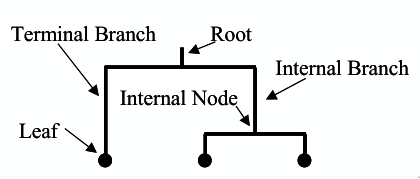
\includegraphics[width=\textwidth]{dendrogram}
		\caption{Dendrogram structure}
		\label{fig:dendrogram}
	\end{figure}

		\subsection{Interpretation}
		Hierarchical clustering sometimes show pattern that are meaningless or spurious.
		So the interpretation of the algorithm has to be performed.

		\subsection{Advantages of hierarchical clustering}

			\subsubsection{Correct number of clusters}
			One advantage of hierarchical clustering is that the correct number of cluster is obtained looking at the dendrogram.

				\begin{figure}[H]
					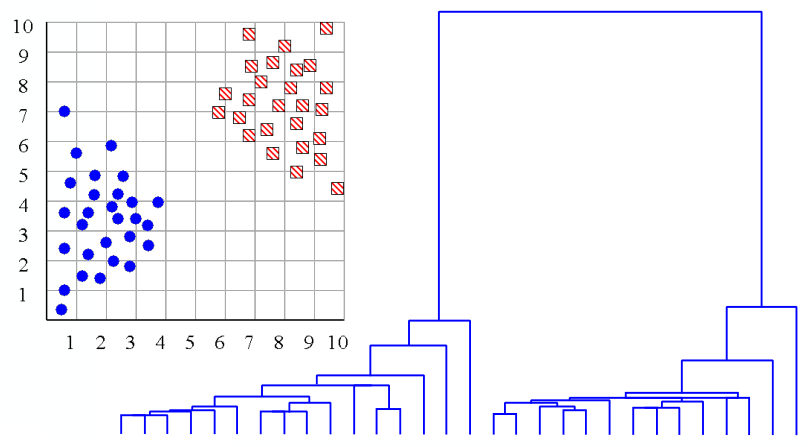
\includegraphics[width=\textwidth]{correct-number}
					\caption{Correct number of clusters}
					\label{fig:correct-number}
				\end{figure}

			\subsubsection{Outliers}
			Moreover when using hierarchical clustering the outliers are easily identified.

			\begin{figure}[H]
				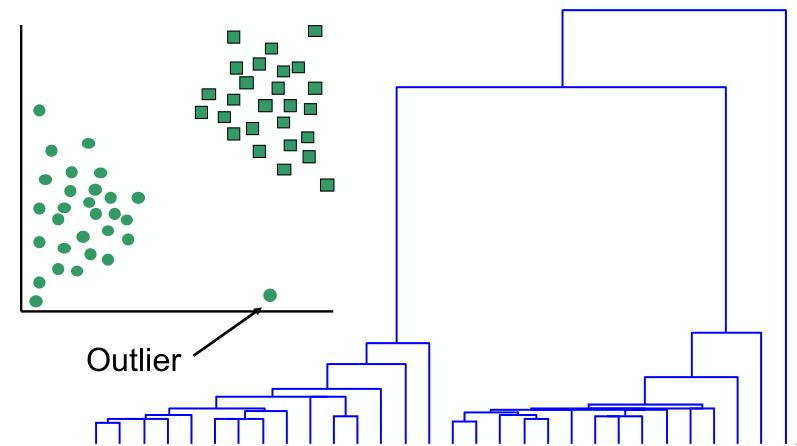
\includegraphics[width=\textwidth]{outliers}
				\caption{Outliers}
				\label{fig:dendrogram}
			\end{figure}

	\subsection{Hierarchical clustering approach}
	The number of dendrograms $D$ with $n$ leafs are:

	$$D = \frac{2n-3)!}{2^{n-2}(n-2)!}$$

	They can be built with two approaches:

	\begin{itemize}
		\item Bottom-up or agglomerative approach: each item is grouped alone into its own cluster and then the best pair to merge into a new cluster is found.
			This is repeated until all clusters are fused together.
		\item Top-down or divisive approach: all the data is grouped into a single cluster, then the best division into two cluster is chosen and this is repeated recursively on both sides.
	\end{itemize}

	\subsection{Summary of hierarchical methods}

	\begin{itemize}
		\item No need to specify the number of clusters in advance.
		\item The hierarchical nature maps nicely onto human intuition for some domains.
		\item They do not scale well: $O(n^2)$.
		\item The interpretation of the results is very subjective.
	\end{itemize}

\section{Partitional clustering}
In partitional clustering each item is placed in exactly one of $K$ non-overlapping clusters.
The number of cluster is provided as input.

	\subsection{K-means}

	\begin{enumerate}
		\item Choose the value $k$.
		\item Initialize the $k$ cluster centres randomly.
		\item Decide the class memberships of the $N$ objects by assigning them to the nearest cluster centre.
		\item Re-estimate the $k$-cluster centres by assuming the memberships found are correct.
		\item If non of the $N$ objects changed memberships in the last iteration exit, otherwise go back to step $3$.
	\end{enumerate}

		\subsubsection{Conclusion}

		\begin{itemize}
			\item Relatively efficient: $O(tkn)$ where $n$ is the number of objects, $k$ is the number of clusters and $t$ the number of iterations.
			\item It often terminates at a local optimum.
			\item It is applicable only when a mean can be defined.
			\item The number of cluster has to be specified in advance.
			\item It is unable to handle noisy data or outliers.
			\item It is not suitable to discover clusters with non-convex shapes.
		\end{itemize}

	\subsection{Sum of squared errors}
	The sum of squared error will be the objective function that determines how well the data is divided into clusters.

	$$SE_{K_i} = \sum\limits_{j=1}^m[D(C_{ij}, C_{K_i})]^2$$

	$$SE_K = \sum\limits_{i=1}^jSE_{K_i}$$

	\subsection{Choosing K}
	The optimal $k$ is the one such that the $\min SE$ is found.
	It can be chosen running the algorithm with iteratively increasing value of $k$ and looking at the Knee or elbow plot of $k$ in relation with $SE$ as in \ref{fig:elbow}.

	\begin{figure}[H]
		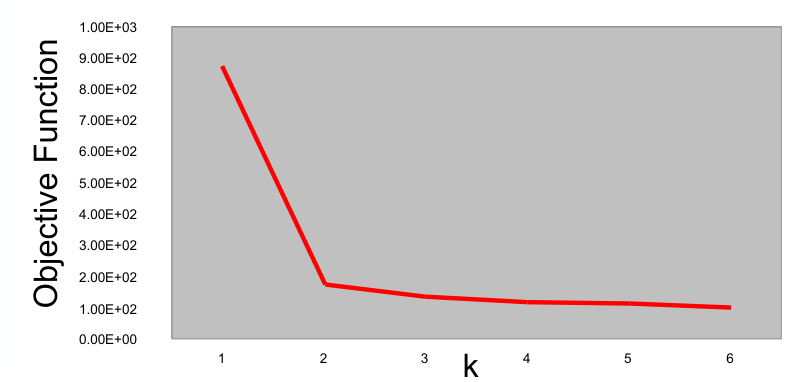
\includegraphics[width=\textwidth]{elbow}
		\caption{Knee or elbow plot}
		\label{fig:elbow}
	\end{figure}

\section{Protein structure networks}
Protein structure networks represents proteins as networks built after the molecular dynamics simulation is performed.

\begin{figure}[H]
	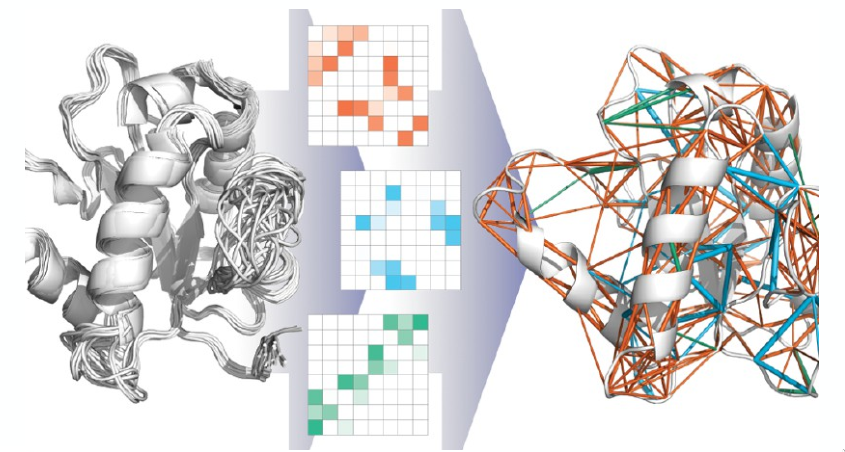
\includegraphics[width=\textwidth]{psn}
	\caption{Protein structure network}
	\label{fig:psn}
\end{figure}

	\subsection{PyInteraph}
	PyInteraph is an algorithm to analyse the trajectories.
	The protein is represented as a graph where the nodes are the side chains of protein residues and the edges can be defined in term of:

	\begin{multicols}{2}
		\begin{itemize}
			\item Distance.
			\item Atomic contacts.
			\item Van der Waals interactions.
			\item Interaction energy.
		\end{itemize}
	\end{multicols}

	Then a graph analysis approach to the intramolecular interaction network IIN is performed.

	\subsection{Classes of interactions}
	This interactions are non-bonded interactions that are not present in the force-field.

		\subsubsection{Hydrophobic contacts}
		In the hydrophobic contacts the centre of mass of the two side chains are distant less than $5\si{\angstrom}$.
		The centres of mass is specified by the force field for different masses, so they will be force-field specific.
		It has default residues, the typically hydrophobic residues that are checked by pyInteraph.

		\begin{multicols}{4}
			\begin{itemize}
				\item Ala.
				\item Ile.
				\item Val.
				\item Phe.
				\item Met.
				\item Trp.
				\item Pro.
			\end{itemize}
		\end{multicols}

		\subsubsection{Salt bridges}
		Salt bridges corresponds to the interaction of groups with opposite charge.
		They are formed between atom pairs belonging to two charged groups of two different residues with distance less than $4.5\si{\angstrom}$.

		\subsubsection{Hydrogen bonds}
		Hydrogen bond happen when the distance between the acceptor and the hydrogen atom is less than $3.5\si{\angstrom}$ and the donor-hydrogen-acceptor angle is greater than $120^\circ$.

	\subsection{Persistence}
	Persitence is the fraction of the number of structures in the ensemble in which the interaction was observed: the interactions are computed for each frame.
	For hydrogen-bond one or more interactions may exist between two residues.
	PyInteraph will generate interaction matrix for each type of interaction.
	Then for each interaction the edge weight is given, corresponding to the persistence value.
	Then these three interaction network are filtered according to a measure providing a persistence threshold.
	When the value of the persistence is higher than the threshold a contact is assumed true.
	After that the macro-intramolecular-interaction network that collects informations about all the different of interactions.

	\subsection{Persistence threshold}
	To choose the persistence threshold the connected components of the protein structure network have to be found.
	A connected component is a subgraph in which a path exists between any two vertices, but no path exist to any other vertices of the main graph: there are no edges connecting two connected components.
	After having obtained them for each value of the persistence, so that a connection is defined whenever the persistence is higher than the value.
	It can be seen how decreasing the threshold the size of the connected components increase.
	A typical graph of persistence over component size a kink can be found and that will be the persistence threshold.

	\subsection{Graph analysis}
	Some analysis provided by pyInteraph are:

	\begin{itemize}
		\item Computing the highly connected residues or hubs: residues with with more than $3$ or $4$ edges.
			A list of hubs and their respective connectivity degree (how many residue are connected to them) is computed.
			Hubs indicates that their residues will play a key role in the structure or function of the protein.
		\item Connected components.
			The groups and part of the protein are connected and can be assumed to behave as rigid object in the protein.
			These can find domains that behave mechanical in the same way in the protein.
		\item Shortest path between two specified residues.
			This is useful because many proteins have allosteric communication pathways and they could be explored by this analysis, finding the amino acids that transport the mechanical signal from one side of the protein to another.
	\end{itemize}

	\subsection{Examples}

		\subsubsection{p53 DNA binding domain}
		Hydrophobic interactions play a crucial role in the stabilization of the protein core and in the maintenance of the 3D structure and stability.
		In general hydrophobic interaction play a crucial role in the folding, structure and function of the protein.

		\begin{figure}[H]
			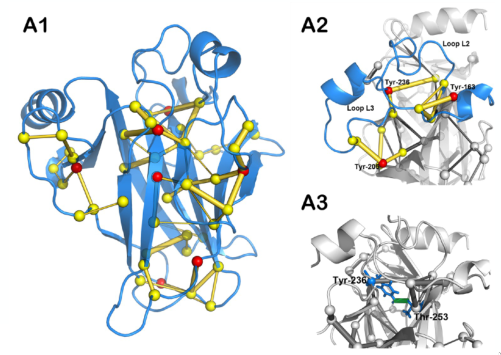
\includegraphics[width=\textwidth]{p53}
			\caption{p53}
			\label{fig:p53}
		\end{figure}

		\subsubsection{Vibrio proteinase (VAP)}
		Salt bridges or hydrogen bonds are highly flexible and cooperatively organized in networks across the protein structure or for temperature adapted organisms.

		\begin{figure}[H]
			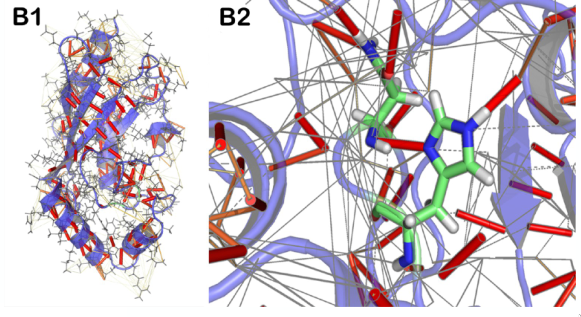
\includegraphics[width=\textwidth]{vap}
			\caption{VAP}
			\label{fig:vap}
		\end{figure}
